\documentclass[letterpaper,11pt]{article}
\oddsidemargin -1.0cm \textwidth 17.5cm

\usepackage[utf8]{inputenc}
\usepackage[activeacute,spanish, es-lcroman]{babel}
\decimalpoint
\usepackage{amsfonts,setspace}
\usepackage{amsmath}
\usepackage{amssymb, amsmath, amsthm}
\usepackage{comment}
\usepackage{float}
\usepackage{amssymb}
\usepackage{dsfont}
\usepackage{anysize}
\usepackage{multicol}
\usepackage{enumerate}
\usepackage{graphicx}
\usepackage[left=1.5cm,top=2cm,right=1.5cm, bottom=1.7cm]{geometry}
\setlength\headheight{1.5em} 
\usepackage{fancyhdr}
\usepackage{multicol}
\usepackage{hyperref}
\usepackage{wrapfig}
\usepackage{subcaption}
\usepackage{siunitx}
\usepackage{cancel}
\usepackage{mdwlist}
\usepackage{svg}
\pagestyle{fancy}
\fancyhf{}
\renewcommand{\labelenumi}{\normalsize\bfseries P\arabic{enumi}.}
\renewcommand{\labelenumii}{\normalsize\bfseries (\alph{enumii})}
\renewcommand{\labelenumiii}{\normalsize\bfseries \roman{enumiii})}


\begin{document}

\fancyhead[L]{\itshape{Facultad de Ciencias F\'isicas y Matem\'aticas}}
\fancyhead[R]{\itshape{Universidad de Chile}}

\begin{minipage}{11.5cm}
    \begin{flushleft}
        \hspace*{-0.6cm}\textbf{FI1000-1 Introducción a la Física Clásica}\\
        \hspace*{-0.6cm}\textbf{Profesor:} Ignacio Bordeu\\
        \hspace*{-0.6cm}\textbf{Auxiliares:} Alejandro Cartes \& Simón Yáñez\\
        \hspace*{-0.6cm}\textbf{Ayudante:} Javier Cubillos\\
    \end{flushleft}
\end{minipage}

\begin{picture}(2,3)
    \put(366, 10){
\includegraphics[scale=0.9]{2020-1/Imágenes/logo/dfi-fcfm.pdf}}
\end{picture}

\begin{center}
	\LARGE\textbf{Auxiliar \#1}\\
	\Large{Trigonometría}
\end{center}

\vspace{-1cm}
\begin{enumerate}\setlength{\itemsep}{0.4cm}

\rfoot[]{pág. \thepage}

\item[]

\item Dos observadores $A$ y $B$ miden ángulos de elevación de un avión que los sobrevuela a una altura constante. En cierto instante los ángulos medidos por $A$ y $B$ son $\alpha = 60^{\circ}$ y $\beta = 40^{\circ}$, respectivamente. La separación entre $A$ y  $B$ es $D = \SI{1}{\km}$. ¿A qué altura vuela el avión?

\begin{figure}[H]
    \centering
    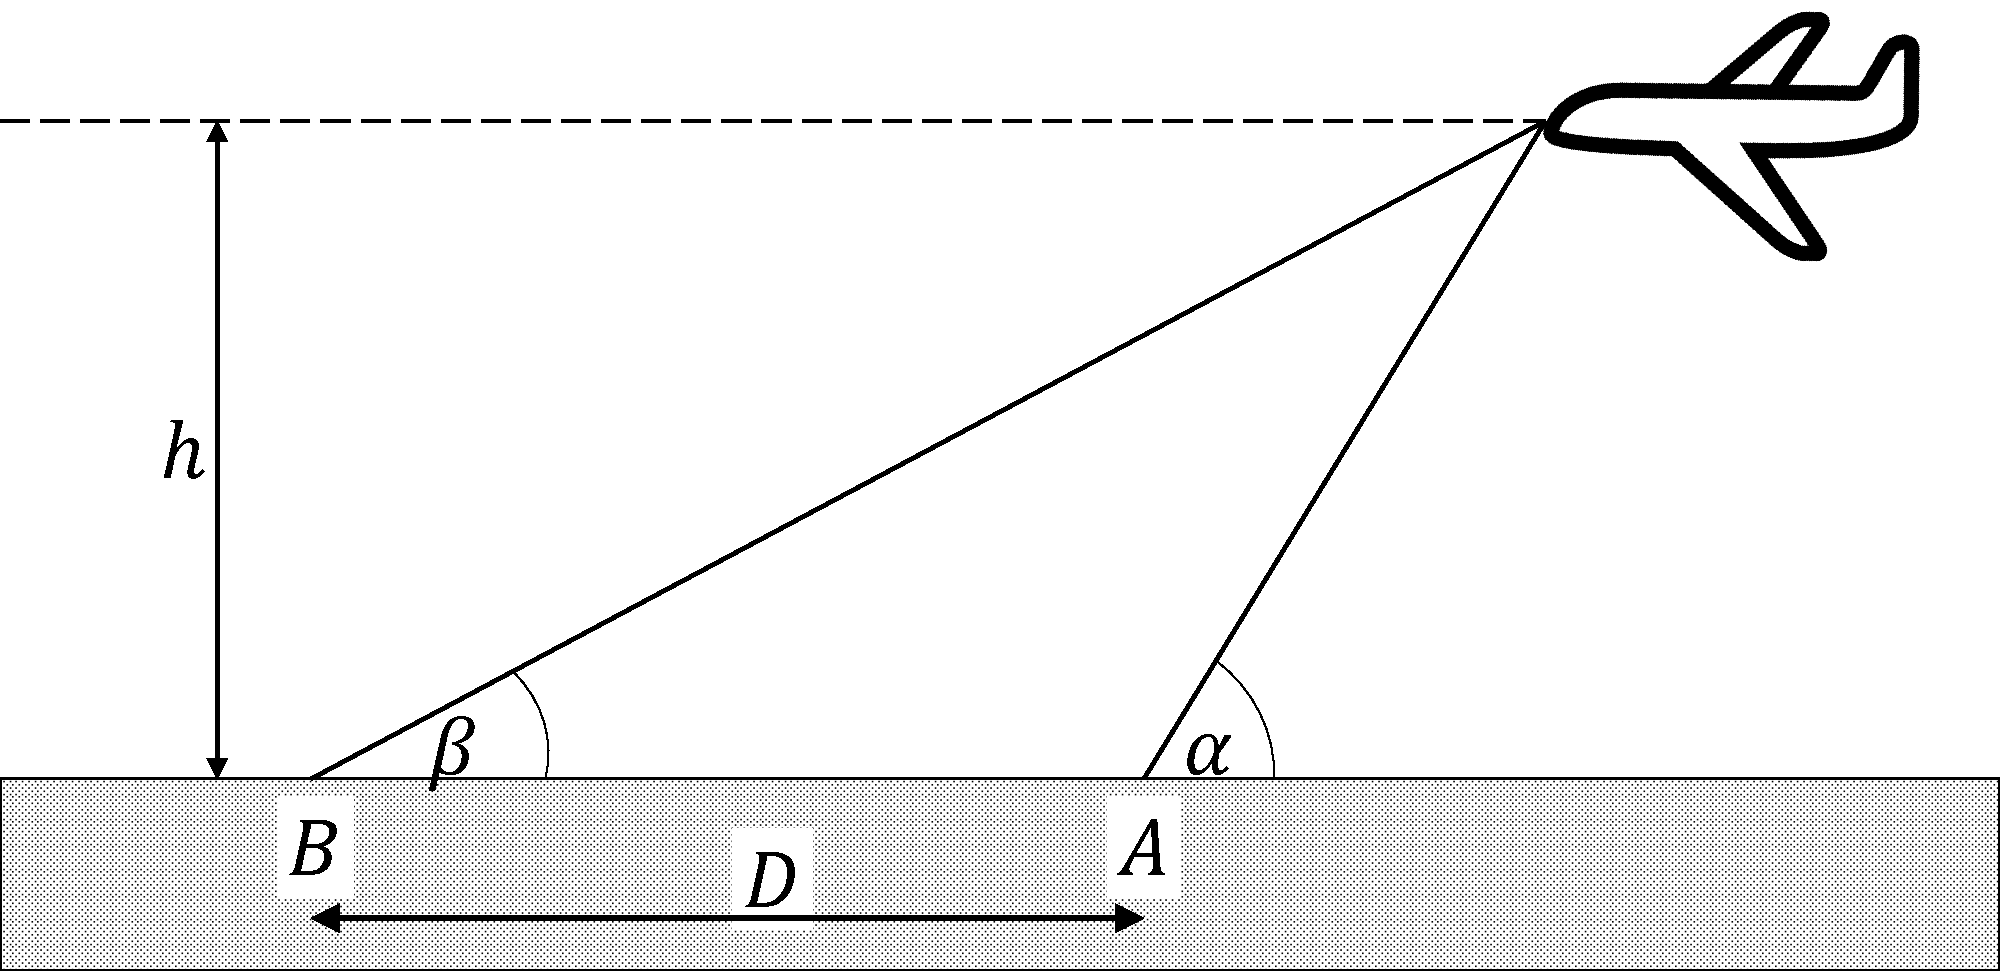
\includegraphics[width=0.35\linewidth]{2021-1/Imagenes/aux0/avion.pdf}
\end{figure}


\item Una tortuga se encuentra al pie de un cerro cuya inclinación es $\gamma$. Desde cierta posición avista, con un ángulo de elevación $\alpha$ respecto al piso, a su compañera tortuga que se encuentra en la punta de un poste vertical ubicado en la cima del cerro. Luego, la tortuga avanza una distancia $d$ en dirección al poste. En este lugar avista a su compañera con un ángulo de elevación $\beta$. Encuentre la altura $h$ del poste en el que se encuentra la compañera tortuga. Analice el caso $\gamma\rightarrow 0$

\begin{figure}[H]
    \centering
        \centering
        \svgpath{../../2021-2/img/aux1}
        \includesvg[width=0.4\linewidth]{tortugas.svg}
\end{figure}




% Para imágenes vectoriales -> el texto tiene que estar en LaTeX
% \begin{figure}[htbp]
%   \centering
%   \svgpath{../Imagenes/ejercicios}  -> .. irse pa'trás 
%   \includesvg{ej5.svg}
% \end{figure}

\end{enumerate}
\end{document}
